%%%%%%%%%%%%%%%%%%%%%%%%%%%%%%%%%%%%%%%%%%%%%%%%%%%%%%%%%%%%%%%%%%%%%%%%
%                                                                      %
%     File: Thesis_Background.tex                                      %
%     Tex Master: Thesis.tex                                           %
%                                                                      %
%     Author: Andre C. Marta                                           %
%     Last modified :  4 Mar 2024                                      %
%                                                                      %
%%%%%%%%%%%%%%%%%%%%%%%%%%%%%%%%%%%%%%%%%%%%%%%%%%%%%%%%%%%%%%%%%%%%%%%%

\chapter{Computational Methods}
\label{chapter:computational_methods}

Insert your chapter material here.

paper \cite{arnold_numerical_2011} book \cite{press_numerical_2007}


\section{Numerical Integration}

\subsection{Runge-Kutta 4th Order for Vehicle Dynamics}

\begin{equation}
    \frac{\mathrm{d}\phi}{\mathrm{d}t} = f(t, \phi)
\end{equation}


general formula

\begin{equation}
    \phi_{n+1} = \phi_{n+1} + \frac{1}{6} k_1 + \frac{1}{3} k_2 + \frac{1}{3} k_3 + \frac{1}{6} k_4 + O(h^5)
\end{equation}


\begin{equation}
    k_1 = f\left(t_n, \phi_n\right) \Delta t
\end{equation}
\begin{equation}
    k_2 = f\left(t_n + \frac{1}{2}\Delta t, \phi_n + \frac{1}{2} k_1\right) \Delta t
\end{equation}
\begin{equation}
    k_3 = f\left(t_n + \frac{1}{2}\Delta t, \phi_n + \frac{1}{2} k_2\right) \Delta t
\end{equation}
\begin{equation}
    k_4 = f\left(t_n + \frac{1}{2}\Delta t, \phi_n + k_3\right) \Delta t
\end{equation}

\subsection{Integration Methods for Blade Loads}

\textcolor{blue}{Simpson's Rule}

\begin{equation}
    \int_\epsilon^{L+\epsilon} \mathbf{F} \,\mathrm{d}y = \frac{h}{3} \left( f_{0} + 4\left(f_{1} + f_{3} + f_{5} + \ldots + f_{2n-1} \right) \right)
\end{equation}


\section{Simulator Development}


\subsection{Simulation flowchart}

\begin{figure}[!htb]
    \centering
    \includegraphics[width=\textwidth]{Figures/comp_method/simulation_flowchart.png}
    \caption{Computational implementation flowchart}
    \label{fig:flowchart}
\end{figure}

\subsection{Application Interface}

\section{Model Validation and Verification}
\label{sec:validation_verification}

For the autorrotation model previous presented, a critical aspect of its performance is to understand the behavior of the system under different conditions. In this section, it will be discuss the validation and verification with the following strategy:

\begin{itemize}
    \item \textbf{1st step:} Validation and verification of the rotor-aerodynamic model with wind tunnel experimental data from \cite{brindejonc_design_2007}. This step consist in validate the \textit{black box} model, i.e. the calcutaion of the rotor force and torque inside the red box in on the flowchart presented in Fig. \ref{fig:flowchart}
    
    \item \textbf{2nd step:} Verification of the dynamic model with 2 sets of simlation data, one provided in \cite{marques_rocket_2022} and the another one presented in \cite{riegler_daedalus_2018}
\end{itemize}

\subsection{Validation and Verification with wind tunnel data}

Brindejonc et al. (2007) \cite{brindejonc_design_2007} conducted wind tunnel experiments to study a rotor under the autorotation phenomena. The experimental setup consisted of a 2-bladed with no pitch-flap coupling and no precone. The rotor characteristics are summed up in Table \ref{tb:geo_paper_validation}

\begin{table}[!htb]
    \centering
    \begin{tabular}{@{}lll@{}}
    \toprule
    \multicolumn{3}{c}{Rotor Geometry} \\ \midrule
    Blade number, $N_b$                   &  & 2           \\
    Rotor diameter, $R_r$ & [\unit{m}]              & 0.33        \\
    Blade span, $S_b$ & [\unit{m}]                  & 0.1524      \\
    Blade chord, $c$ & [\unit{m}]                 & 0.0287      \\
    Blade twist, $\frac{\mathrm{d}\theta}{\mathrm{d}S_b}$ & [\unit{m}]                 & 0           \\
    Blade pitch angle, $\theta$ & [\unit{\degree / m}] & -6, -8, -12 \\
    Airfoil                               &  & NACA 0010   \\ \bottomrule
    \end{tabular}\
    \caption[Wind tunnel rotor geometric characteristics]{Wind tunnel rotor geometric characteristics, \cite{brindejonc_design_2007}}
    \label{tb:geo_paper_validation}
\end{table}

Considering the wind tunnel data \cite{brindejonc_design_2007}, it is possible to simulate a set of diferente experimental test cases. {In \cite{brindejonc_design_2007} is presented two plots from which the following parameteres of the rotor state can be taken: the rotor's speed, the rotor's thrust force and wind velocity for all the differente pitch angles in Table \ref{tb:geo_paper_validation}. So, verify the rotor-aerodynamic model, the criterion used is the comparison between the simulated and experimental values is rotor's thrust force. However, for computing the rotor's perfomance, is still needed the rotor's induced velocity, which can be estimate with the Linear Momentum Theory \cite{leishman_principles_2006}

\begin{equation}
    v_i = \frac{T ^ {\frac{3}{2}}}{\sqrt{2 \rho A_r }},
\end{equation}

where $T$ is the trust force in \unit{N}, $\rho$ the air density in \unit{Kg/m^3} and $A$ the rotor's disk area in \unit{m^2}. 

To make a comparison, the thrust error is computed in percentage \unit{\%} as

\begin{equation}
    \mathrm{e} =\frac{|T_{mode} - T_{paper}|}{T_{paper}}
\end{equation}

So, from the paper, the results can be compiled in the following table


\begin{table}[!htb]
    \centering
    \begin{tabular}{@{}llll|l|lll@{}}
        \toprule
        \multicolumn{4}{c|}{Paper Data}       & \multicolumn{1}{c|}{Estimation} & \multicolumn{3}{c}{Present Work} \\ \midrule
        $\theta$ [\unit{\deg}] &  $V_\infty$ [\unit{m/s}] & $RPM$ & $F_z$ [\unit{N}]& $v_i$ [\unit{m/s}] & $F_z$ [\unit{N}] & $T$ [\unit{N/m}] & $e$ [\%]\\ \midrule
        -6 & -2 & 700.59 & 0.162 & -0.649 & 0.151 & 0.018 & 6.5 \\
        -6 & -4 & 1573.23 & 0.675 & -1.680 & 0.751 & 0.091 & 11.3 \\
        -6 & -8 & 3322.39 & 2.687 & -4.222 & 3.218 & 0.390 & 19.7 \\
        -8 & -2 & 619.54 & 0.127 & -0.553 & 0.127 & 0.016 & 0.6 \\
        -8 & -4 & 1370.03 & 0.451 & -1.286 & 0.630 & 0.077 & 39.5 \\
        -8 & -8 & 2791.17 & 1.701 & -3.113 & 2.614 & 0.319 & 53.7 \\
        -12 & -2 & 550.48 & 0.067 & -0.360 & 0.099 & 0.012 & 47.9 \\
        -12 & -4 & 1063.95 & 0.269 & -0.911 & 0.372 & 0.046 & 38.4 \\
        -12 & -8 & 2224.33 & 0.976 & -2.149 & 1.675 & 0.206 & 71.6 \\
        \bottomrule
    \end{tabular}
    \caption{resultsD ATA}
\end{table}


\begin{figure}[!htb]
    \centering
    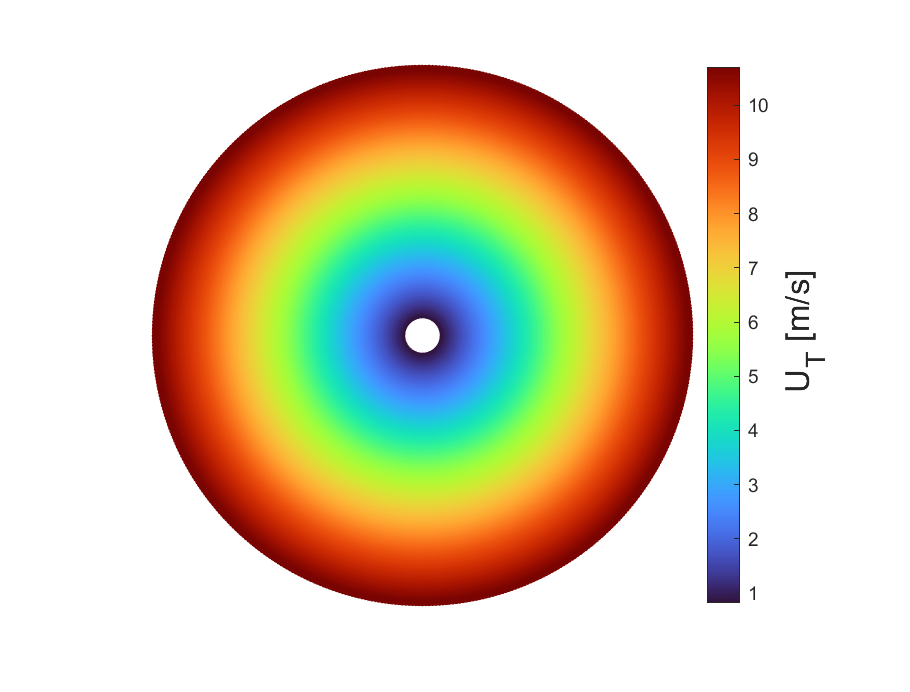
\includegraphics[width=0.49\textwidth]{Figures/comp_method/sim_B/U_T.eps}
    \caption[Tangencial Velocity]{Tangencial Velocity}
    \label{fig:ASDASDA}
\end{figure}

\begin{figure}[!htb]
    \centering
    \begin{minipage}{.49\textwidth}
      \centering
      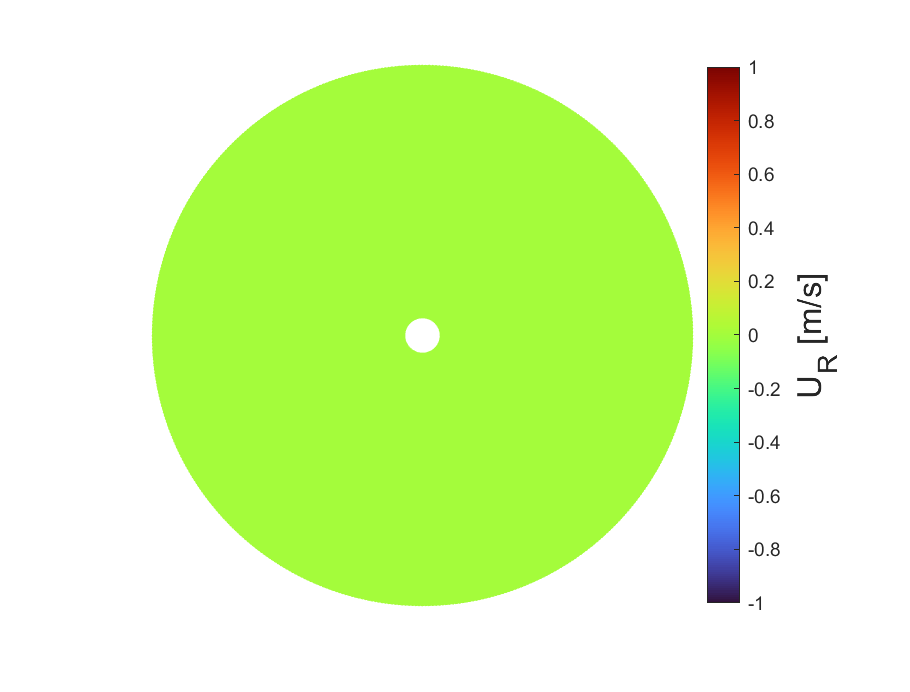
\includegraphics[width=\textwidth]{Figures/comp_method/sim_B/U_R.eps}
      \caption[Radial Velocity]{Radial Velocity}
      \label{fig:imagem1}
    \end{minipage}%
    \begin{minipage}{.01\textwidth}
         \hfill
    \end{minipage}
    \begin{minipage}{.49\textwidth}
      \centering
      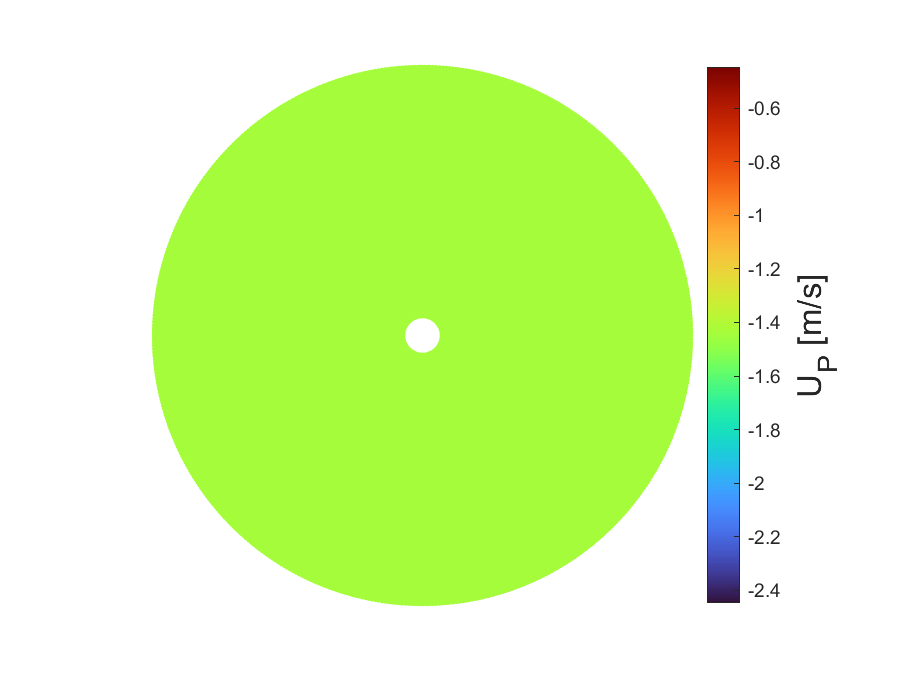
\includegraphics[width=\textwidth]{Figures/comp_method/sim_B/U_P.eps}
      \caption[Vertical Velocity]{Vertical Velocity}
      \label{fig:imagem3}
    \end{minipage}
\end{figure}

\begin{figure}[!htb]
    \centering
    \begin{minipage}{.49\textwidth}
      \centering
      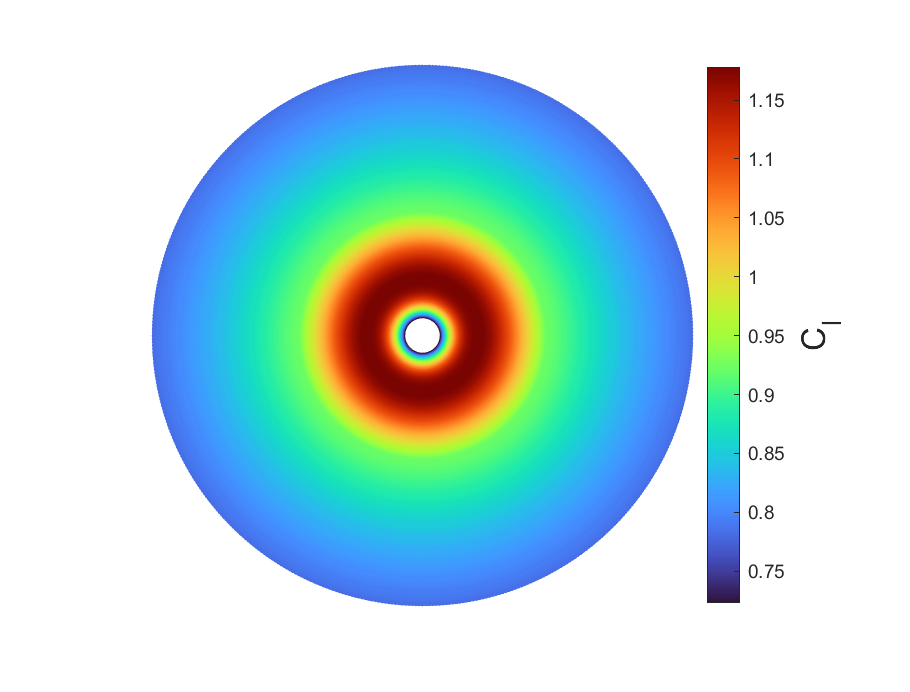
\includegraphics[width=\textwidth]{Figures/comp_method/sim_B/cl.eps}
      \caption[Lift Coefficient]{Lift Coefficient}
      \label{fig:imagem111}
    \end{minipage}%
    \begin{minipage}{.01\textwidth}
         \hfill
    \end{minipage}
    \begin{minipage}{.49\textwidth}
      \centering
      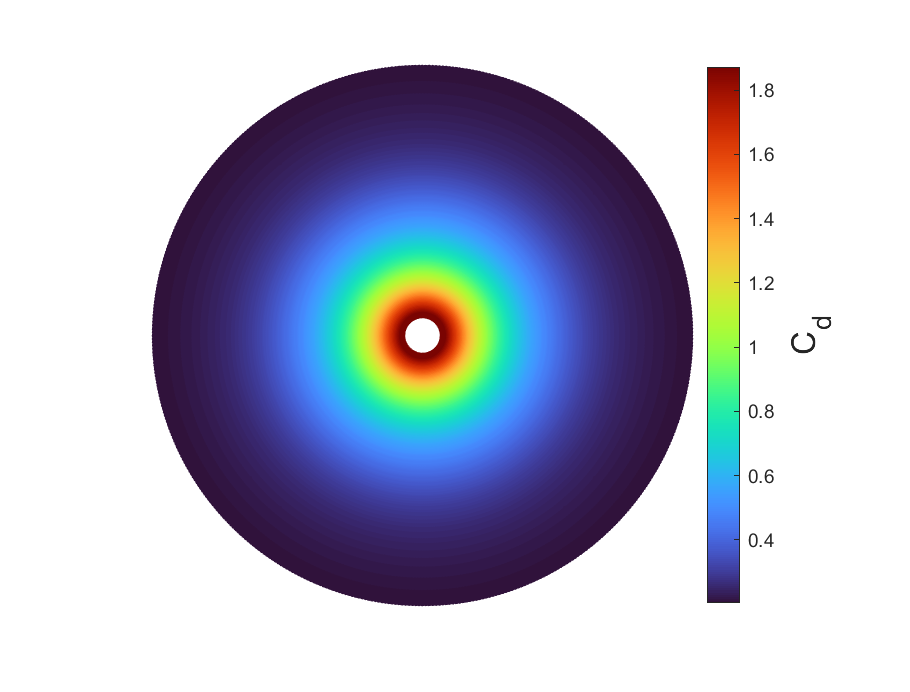
\includegraphics[width=\textwidth]{Figures/comp_method/sim_B/cd.eps}
      \caption[Incidence angle]{Incidence Angle}
      \label{fig:imagem311}
    \end{minipage}
\end{figure}


\begin{figure}[!htb]
    \centering
    \begin{minipage}{.49\textwidth}
      \centering
      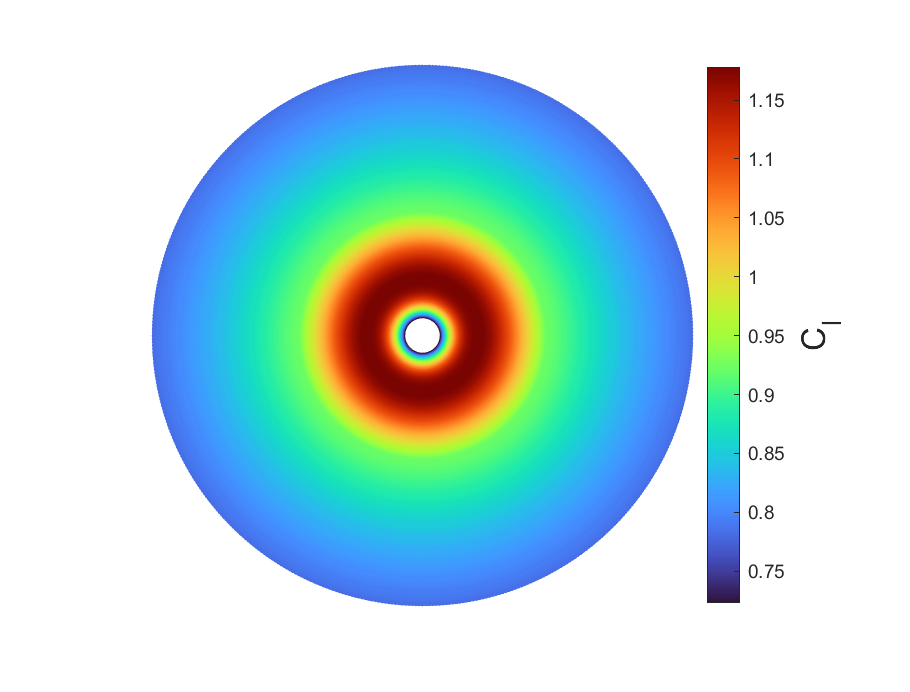
\includegraphics[width=\textwidth]{Figures/comp_method/sim_B/cl.eps}
      \caption[Lift Coefficient]{Lift Coefficient}
      \label{fig:imagem11}
    \end{minipage}%
    \begin{minipage}{.01\textwidth}
         \hfill
    \end{minipage}
    \begin{minipage}{.49\textwidth}
      \centering
      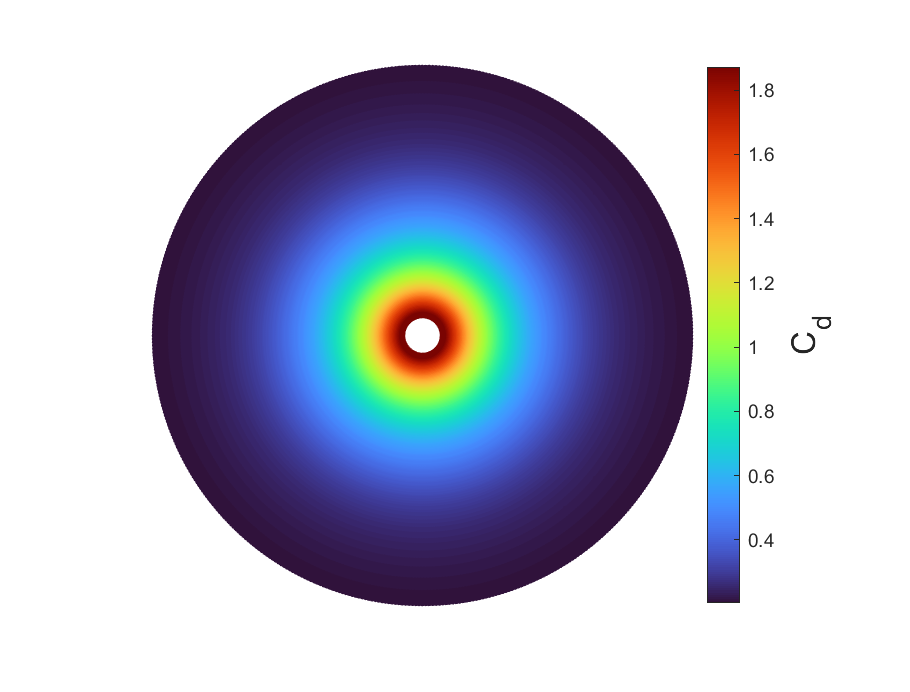
\includegraphics[width=\textwidth]{Figures/comp_method/sim_B/cd.eps}
      \caption[Drag Coefficient]{Drag Coefficient}
      \label{fig:imagem31}
    \end{minipage}
\end{figure}


\subsection{Project Daedalus}


\subsection{Previous Work Comparison}


\section{Mesh Study}

On this section, the mesh study is presented where three key points are discussed: 1) the time step for the dynamic model solver, 2) the azimutal rotor's distribution and 3) the blade element discretization for \gls{bet}.

\subsection{Time Step}

\subsection{Azimtutal Distribution}

\subsection{Blade Discretization}